\documentclass[10pt,twocolumn]{article}

\usepackage[margin=0.68in,columnsep=0.22in]{geometry}
\usepackage[T1]{fontenc}
\usepackage[utf8]{inputenc}
\usepackage{lmodern}
\usepackage{microtype}
\usepackage{amsmath,amssymb}
\usepackage{graphicx}
\usepackage{booktabs}
\usepackage{tabularx}
\usepackage{array}
\usepackage{xcolor}
\usepackage[font=small,labelfont=bf,skip=4pt]{caption}
\usepackage[numbers,sort&compress]{natbib}
\usepackage[colorlinks=true,linkcolor=blue!55!black,citecolor=blue!55!black,urlcolor=blue!55!black]{hyperref}

% Compact section heading spacing (standard LaTeX kernel, no extra packages)
\makeatletter
\renewcommand\section{\@startsection{section}{1}{\z@}%
  {-1.5ex \@plus -0.5ex \@minus -0.2ex}%
  {0.7ex \@plus 0.2ex}%
  {\normalfont\large\bfseries}}
\renewcommand\subsection{\@startsection{subsection}{2}{\z@}%
  {-1.1ex \@plus -0.3ex \@minus -0.1ex}%
  {0.4ex \@plus 0.1ex}%
  {\normalfont\normalsize\bfseries}}
\makeatother

% Compact float spacing
\setlength{\textfloatsep}{8pt plus 2pt minus 2pt}
\setlength{\dbltextfloatsep}{9pt plus 2pt minus 2pt}
\setlength{\floatsep}{6pt plus 2pt minus 2pt}
\setlength{\dblfloatsep}{7pt plus 2pt minus 2pt}

\newcommand{\code}[1]{\texttt{\small #1}}
\newcommand{\stage}[1]{\texttt{\footnotesize #1}}

\title{\vspace{-1.4em}\Large\bfseries From Naive PyTorch to Surpassing vLLM: A Profile-Guided Empirical Study of LLM Inference Optimization on Consumer Blackwell GPUs}

\author{\normalsize shin-x-nihs \\[0.25em]
\small Code: \href{https://github.com/shin-x-nihs/mini-inference-stack}{github.com/shin-x-nihs/mini-inference-stack} \quad|\quad
Interactive Dashboard: \href{https://shin-x-nihs.github.io/mini-inference-stack/}{shin-x-nihs.github.io/mini-inference-stack}}

\date{\vspace{-1.4em}}

\begin{document}
\maketitle

\begin{abstract}
Large language model (LLM) serving performance is governed by rapidly shifting bottlenecks across algorithmic complexity, memory hierarchy, GPU occupancy, request scheduling, and host-side kernel dispatch. Production serving engines bundle dozens of optimizations together, obscuring individual causal effects and non-obvious bottleneck inversions—particularly on bandwidth- and thermally-constrained consumer GPUs. We present a reproducible, dual-track empirical systems study of \code{Qwen2.5-Coder-1.5B-Instruct} (\code{bfloat16}) on a single NVIDIA GeForce RTX 5080 Laptop GPU (Blackwell, \code{sm\_120}), combining closed-loop concurrency and context-length benchmarks with hardware-level attribution via Nsight Systems (\code{nsys}) and Nsight Compute (\code{ncu}). In our strictly additive custom engine track (Stages~0$\rightarrow$6), adding one architectural optimization per stage under 100\% greedy token parity improves single-stream ($C{=}1$) throughput by $7.60\times$ ($14.93 \rightarrow 113.42$~tok/s), $C{=}16$ throughput by $72.93\times$ ($14.61 \rightarrow 1{,}065.51$~tok/s), and $L{=}2048$ decode TPOT by $31.95\times$ ($265.51 \rightarrow 8.31$~ms). Stage~6 (Triton FlashAttention-2, Split-K decode, paged KV cache, continuous batching, fused Triton operators, and bucketed CUDA graphs) surpasses baseline vLLM~0.31.0 at every tested concurrency ($1{,}770.61$ vs.\ $1{,}232.26$~tok/s and $9.39\times$ tighter P99 ITL at $C{=}64$) and every context length $L \in [128, 8192]$. In our parallel vLLM feature-isolation track, we quantify why draft-model speculative decoding regresses $-20\%$ to $-29\%$ at $C \ge 4$ despite a $15.5\times$ decode arithmetic-intensity jump, whereas automatic prefix caching boosts $C{=}64$ throughput by $+133.3\%$ to $2{,}874.36$~tok/s.
\end{abstract}

% ============================================================================
\section{Introduction}
% ============================================================================
Modern LLM inference engines such as vLLM~\cite{kwon2023vllm} and SGLang~\cite{zheng2024sglang} achieve high throughput and low latency by simultaneously combining FlashAttention~\cite{dao2022flashattention,dao2024flashattention2}, PagedAttention~\cite{kwon2023vllm}, iteration-level continuous batching~\cite{yu2022orca}, fused Triton/CUDA operators~\cite{tillet2019triton}, and CUDA graphs. While highly effective in production, evaluating these mechanisms only inside a monolithic runtime makes it difficult to attribute end-to-end speedups to specific hardware bottlenecks or to observe how eliminating one bottleneck immediately exposes—or even amplifies—the next. This gap is especially pronounced on consumer laptop GPUs, where lower memory bandwidth, thermal power limits, and WSL2/host-dispatch latencies shift optimization trade-offs compared to datacenter Hopper/Blackwell nodes.

Rather than proposing a new production framework to replace vLLM, this paper presents an honest, profile-guided empirical systems study (\code{mini-inference-stack}) designed around a strict scientific loop: \emph{measure a baseline, attribute host and device bottlenecks using Nsight Systems (\code{nsys}) and Nsight Compute (\code{ncu}), apply exactly one architectural change, verify bit-level greedy token parity, and re-measure}. We organize our investigation into two complementary tracks on a single NVIDIA Blackwell consumer GPU (RTX~5080 Laptop, \code{sm\_120}):
\begin{itemize}\setlength{\itemsep}{1pt}\setlength{\parskip}{0pt}
  \item \textbf{Track B (Strictly Additive Custom Engine, Stages~0$\rightarrow$6):} Seven self-contained stages progressing from naive eager PyTorch to a Triton + Paged-KV + Continuous-Batching + Bucketed-CUDA-Graph engine, demonstrating how eliminating algorithmic, memory-hierarchy, occupancy, and host-dispatch bottlenecks enables a lean custom engine to surpass baseline vLLM~0.31.0 across all tested concurrency and context regimes.
  \item \textbf{Track A (vLLM Feature Isolation, Stages~0$\rightarrow$2):} Controlled single-feature evaluations on vLLM~0.31.0 isolating draft-model speculative decoding~\cite{leviathan2023speculative,chen2023speculative} and automatic prefix caching (RadixAttention)~\cite{zheng2024sglang} against the same frozen baseline.
  \item \textbf{Full-Stack Roofline \& Timeline Attribution:} Cross-stage synthesis linking end-to-end throughput/tail-latency shifts directly to \code{nsys} CPU launch overhead, GPU idle fractions, and \code{ncu} Layer~0 roofline movement~\cite{williams2009roofline}.
\end{itemize}

% ============================================================================
\section{Methodology \& System Architecture}
% ============================================================================

\begin{figure*}[t]
  \centering
  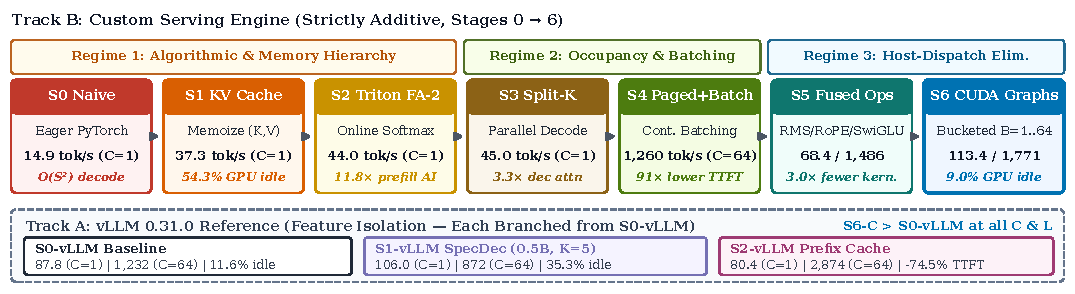
\includegraphics[width=\textwidth]{figures/fig0_progression.pdf}
  \caption{Dual-track experimental architecture of \code{mini-inference-stack}. Track~B (\code{custom-serving/}) adds one architectural optimization per stage across three bottleneck regimes; Track~A (\code{vllm-reference/}) isolates serving-level features directly from frozen \stage{stage-0-vllm}.}
  \label{fig:progression}
\end{figure*}

\subsection{Hardware, Model \& Workload Protocol}
All ten evaluated stages run on a single host under a frozen \code{config.yaml}: an NVIDIA GeForce RTX~5080 Laptop GPU (16~GB GDDR7, Blackwell \code{sm\_120}) with hardware roofline ceilings of $896.0$~GB/s physical DRAM bandwidth and $40.0$~TFLOP/s BF16 Tensor Core compute (ridge point $44.64$~FLOP/B)~\cite{williams2009roofline}. The software stack comprises Windows~11 + WSL2 (Ubuntu~24.04), CUDA~13.1 (\code{nvcc 13.1.80}), Python~3.12, PyTorch~\code{2.13.0+cu130}, Triton~3.7.1~\cite{tillet2019triton}, and vLLM~0.31.0.

The target model is \code{Qwen/\allowbreak Qwen2.5-Coder-1.5B-Instruct}~\cite{hui2024qwen25coder,yang2024qwen25} in \code{bfloat16} (${\sim}1.54$B parameters, $2.907$~GB weights): 28 Transformer layers, 12 query heads, 2 key/value heads (6:1 Grouped-Query Attention~\cite{ainslie2023gqa}), $\text{head\_dim}{=}128$, $\text{hidden\_size}{=}1536$, $\text{rope\_theta}{=}10^6$~\cite{su2024roformer}, RMSNorm~\cite{zhang2019rmsnorm}, SwiGLU MLP~\cite{shazeer2020glu}, tied \code{lm\_head}, and $\text{max\_model\_len}{=}9216$. For \stage{stage-1-vllm} speculative decoding only, we pair this target with \code{Qwen2.5-Coder-0.5B-Instruct} (${\sim}0.49$B, \code{bfloat16}, $K{=}5$).

Every engine implements an identical OpenAI-compatible streaming \code{POST /v1/chat/completions} SSE contract on \code{127.0.0.1:8000}, honouring \code{ignore\_eos} and emitting final \code{usage} chunks. We evaluate four standardized protocols via \code{vllm bench serve} and NVIDIA profilers:
\begin{enumerate}\setlength{\itemsep}{1pt}\setlength{\parskip}{0pt}
  \item \textbf{Concurrency (Pareto) Sweep:} Fixed Python code prompt sized to 512 input / 128 output tokens, greedy decoding ($\text{temperature}{=}0.0$, $\text{seed}{=}42$), across $C \in \{1, 2, 4, 8, 16, 32, 64\}$ (serialized custom Stages~0--3 capped at $C \le 16$). Reports output throughput, mean TPOT, P50/P90/P99 ITL, and mean/P99 TTFT.
  \item \textbf{Context-Length Sweep:} Single-stream ($C{=}1$), $L \in \{128, 256, 512, 1024, 2048, 4096, 8192\}$ input / 64 output tokens, $N{=}10$ prompts (Stages~0--3 capped at $L \le 2048$).
  \item \textbf{Nsight Systems (\code{nsys}):} Live server timeline capture (excluding startup) at $C{=}1$, 1024 input / 64 output tokens, extracting wall time, kernel counts, CPU launch calls and overhead, CUDA graph launches, GPU active/idle union intervals, and per-phase operator breakdown (via NVTX ranges on custom stages and GPU kernel timeline split on vLLM).
  \item \textbf{Nsight Compute (\code{ncu}):} Standalone Layer~0 profiling (server stopped to eliminate VRAM contention) for Prefill ($L{=}2048$) and Decode ($M{=}1$, or $M{=}K{+}1{=}6$ verification in \stage{stage-1-vllm}), recording kernel duration, DRAM bandwidth, arithmetic intensity, occupancy, and attained TFLOP/s (with tensor FLOPs estimated as $\text{inst} \times 4096$).
\end{enumerate}

\subsection{Correctness \& Parity Discipline}
Before any custom stage is benchmarked, \code{custom-serving/test\_parity.py} validates single-step prefill logits against HuggingFace \code{AutoModelForCausalLM} (\code{eager} tolerance $0.0625$ for Stages~0--1; \code{sdpa} tolerance $0.21875$ for Stages~2--6) and verifies $32/32$ (100\%) exact greedy token-ID parity. Stages~4--6 additionally pass batched ($B{=}4$), padded-lane ($B{=}3 \rightarrow \text{bucket } B{=}4$), and KV block reclamation ($256/256$ free blocks) tests. Every recorded benchmark sweep completed with \code{failed = 0}.

\subsection{Seven-Stage Additive Architecture Overview}
Figure~\ref{fig:progression} summarizes the dual-track design. Track~B groups its seven strictly additive stages into three macro-regimes: \emph{Algorithmic \& Memory Hierarchy} (Stages~0$\rightarrow$2), \emph{Occupancy \& Continuous Batching} (Stages~3$\rightarrow$4), and \emph{Host-Dispatch Elimination} (Stages~5$\rightarrow$6). Each stage copies stage $N{-}1$ and introduces a single architectural upgrade, exposing the exact bottleneck transition to stage $N{+}1$.

% ============================================================================
\section{Profile-Guided Progression \texorpdfstring{(S0 $\rightarrow$ S6)}{(S0 to S6)}}
% ============================================================================

Table~\ref{tab:master} compiles the verified end-to-end concurrency, context-scaling, and \code{nsys} profiling metrics across all ten stages. Figures~\ref{fig:pareto}--\ref{fig:roofline} visualize the resulting Pareto frontier, context scaling, host-dispatch decomposition, and Layer~0 hardware roofline.

\begin{table*}[t]
\centering
\caption{Master cross-stage benchmark and Nsight Systems summary across all 10 stages (100\% verified from JSON; \code{failed = 0}). Concurrency sweep uses 512-in/128-out greedy prompts; context sweep uses $C{=}1$, 64-out ($N{=}10$); \code{nsys} captures $C{=}1$, 1024-in/64-out. Best custom/vLLM values highlighted.}
\label{tab:master}
\scriptsize
\setlength{\tabcolsep}{3.4pt}
\begin{tabular}{@{}l rrr rrr rr rrr@{}}
\toprule
& \multicolumn{3}{c}{\textbf{Pareto $C{=}1$ (512/128)}} & \multicolumn{3}{c}{\textbf{Pareto $C{=}64$ ($C{=}16$ for S0--S3)}} & \multicolumn{2}{c}{\textbf{Context $L{=}2048$}} & \multicolumn{3}{c}{\textbf{Nsight Systems ($C{=}1$, 1024/64)}} \\
\cmidrule(lr){2-4} \cmidrule(lr){5-7} \cmidrule(lr){8-9} \cmidrule(lr){10-12}
\textbf{Stage} & \textbf{Tput} & \textbf{TPOT} & \textbf{P99 ITL} & \textbf{Tput} & \textbf{TPOT} & \textbf{P99 ITL} & \textbf{TTFT} & \textbf{TPOT} & \textbf{CPU Calls} & \textbf{Idle} & \textbf{Dec Step} \\
& (tok/s) & (ms) & (ms) & (tok/s) & (ms) & (ms) & (ms) & (ms) & (count) & (\%) & (ms) \\
\midrule
\stage{stage-0-vllm}   & 87.77 & 10.90 & 14.52 & 1,232.26 & 45.15 & 258.96 & 208.14 & 10.11 & 1,636 & 11.61 & 10.67 \\
\stage{stage-1-vllm}   & 105.97 & 8.38 & 69.09 & 872.47 & 59.06 & 392.65 & 411.56 & 10.58 & 19,843 & 35.27 & 8.83 \\
\stage{stage-2-vllm}   & 80.35 & 12.24 & 15.19 & \textbf{2,874.36} & \textbf{20.57} & 44.42 & \textbf{114.36} & 13.60 & 1,636 & 13.09 & 8.69 \\
\midrule
\stage{stage-0-custom} & 14.93 & 66.84 & 109.40 & 14.61$^\dagger$ & 68.44$^\dagger$ & 109.48$^\dagger$ & 275.87 & 265.51 & 85,248 & 8.87 & 110.38 \\
\stage{stage-1-custom} & 37.33 & 26.42 & 57.11 & 37.66$^\dagger$ & 26.27$^\dagger$ & 69.00$^\dagger$ & 330.14 & 24.09 & 85,058 & 54.34 & 21.54 \\
\stage{stage-2-custom} & 43.97 & 22.44 & 49.11 & 40.52$^\dagger$ & 24.44$^\dagger$ & 54.62$^\dagger$ & 196.17 & 22.12 & 72,455 & 39.24 & 25.19 \\
\stage{stage-3-custom} & 44.98 & 21.93 & 52.82 & 38.67$^\dagger$ & 25.65$^\dagger$ & 63.70$^\dagger$ & 190.76 & 21.15 & 74,220 & 59.19 & 24.11 \\
\stage{stage-4-custom} & 38.51 & 25.70 & 45.47 & 1,260.39 & 38.92 & 52.30 & 207.26 & 23.65 & 72,932 & 53.53 & 19.68 \\
\stage{stage-5-custom} & 68.44 & 14.19 & 28.68 & 1,486.13 & 31.71 & 39.64 & 202.66 & 12.20 & 24,100 & 28.97 & 12.58 \\
\stage{stage-6-custom} & \textbf{113.42} & \textbf{8.43} & \textbf{11.88} & \textbf{1,770.61} & \textbf{25.91} & \textbf{27.57} & 174.38 & \textbf{8.31} & \textbf{476} & \textbf{9.03} & \textbf{8.64} \\
\bottomrule
\multicolumn{12}{@{}l@{}}{\scriptsize $^\dagger$Serialized Stages~0--3 were capped at $C{=}16$; at $C{=}16$, \stage{stage-4/5/6-custom} reach $525.85 / 748.22 / 1{,}065.51$~tok/s vs.\ \stage{stage-0-vllm}'s $831.19$~tok/s.}
\end{tabular}
\end{table*}

\begin{figure*}[t]
  \centering
  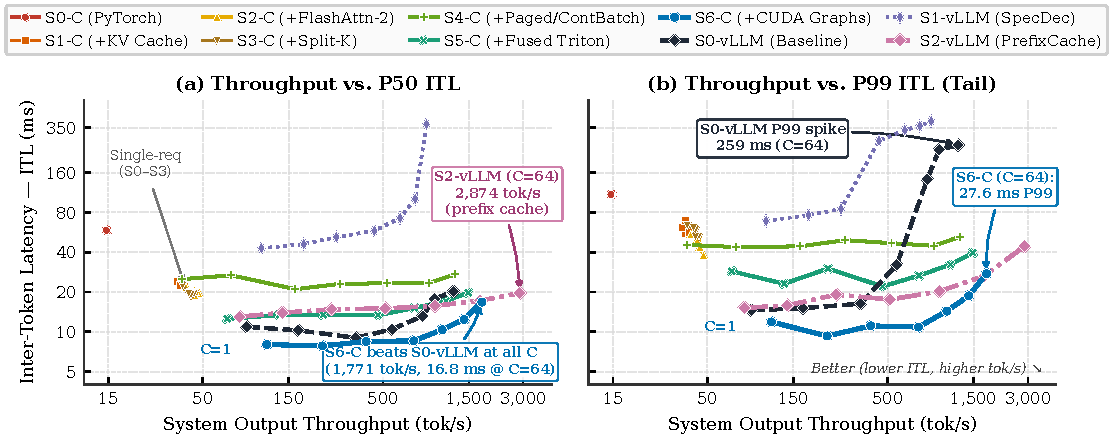
\includegraphics[width=\textwidth]{figures/fig1_pareto.pdf}
  \caption{Throughput vs.\ inter-token latency Pareto frontier across concurrencies $C \in \{1..64\}$ (512-in/128-out greedy). \textbf{(a)}~P50 ITL shows \stage{stage-6-custom} surpassing \stage{stage-0-vllm} at every $C$, while \stage{stage-2-vllm} prefix caching extends the upper bound to $2{,}874$~tok/s. \textbf{(b)}~P99 ITL highlights \stage{stage-6-custom}'s $9.39\times$ tighter tail latency at $C{=}64$ ($27.57$ vs.\ $258.96$~ms).}
  \label{fig:pareto}
\end{figure*}

\subsection{Algorithmic \& Memory-Hierarchy Bottlenecks \texorpdfstring{(S0 $\rightarrow$ S2)}{(S0 to S2)}}
\textbf{Stage~0 $\rightarrow$ Stage~1 (KV Cache).}
\stage{stage-0-custom} implements naive eager PyTorch: loading \code{.safetensors} weights, computing explicit $(Q K^\top)/\sqrt{d}$ attention with \code{repeat\_interleave} for GQA, serializing requests via a global \code{asyncio.Lock}, and recomputing the full sequence on every decode token ($O(S^2)$ work per step). In \code{nsys}, decode consumes $6{,}954.07$~ms out of $7{,}119.30$~ms total wall time ($97.7\%$, $110.38$~ms/step), keeping the GPU $91.13\%$ active purely on redundant recomputation. In the context sweep (Figure~\ref{fig:context}b), doubling $L$ from $512 \rightarrow 1024 \rightarrow 2048$ more than doubles TPOT ($52.68 \rightarrow 120.72 \rightarrow 265.51$~ms, collapsing throughput to $3.76$~tok/s). Because \code{nsys} conclusively isolated $O(S^2)$ recomputation, standalone \code{ncu} was deferred for Stage~0.

\stage{stage-1-custom} adds a per-layer unexpanded $(K, V)$ cache (\code{[B, 2, S, 128]}) with offset RoPE, reducing decode to $M{=}1$ projection ($O(S)$ per step). Decode step time drops $5.12\times$ ($110.38 \rightarrow 21.54$~ms), $C{=}1$ throughput rises $2.50\times$ ($14.93 \rightarrow 37.33$~tok/s), and $L{=}2048$ TPOT plunges $11.02\times$ ($265.51 \rightarrow 24.09$~ms), flattening TPOT across $L \in [128, 2048]$ ($22.56$--$24.27$~ms). Crucially, this triggers our first \emph{bottleneck inversion}: GPU active time drops $8.49\times$ ($6{,}487.79 \rightarrow 764.32$~ms), flipping GPU idle from $8.87\%$ to $54.34\%$ as $85{,}058$ eager launches burn $647.04$~ms on the CPU. Simultaneously, Layer~0 \code{ncu} exposes a severe memory-hierarchy bottleneck in unfused prefill attention: the $Q K^\top$ BMM attains only $135.42$~FLOP/B ($12.0\times$ below \stage{stage-0-vllm}'s $1{,}631.02$~FLOP/B) and is followed by unfused scaling ($453.98~\mu$s), causal masking ($662.91~\mu$s), fp32 casting ($787.58~\mu$s), and \code{softmax\_warp\_forward} ($1{,}012.48~\mu$s at $375.65$~GB/s), totaling $>4{,}100~\mu$s per layer.

\textbf{Stage~1 $\rightarrow$ Stage~2 (Triton FlashAttention-2).}
\stage{stage-2-custom} replaces eager attention with a custom Triton FlashAttention-2~\cite{dao2024flashattention2} forward kernel (\code{\_flash\_attention\_fwd}) using SRAM tiling ($\text{BLOCK\_M}{=}64$ prefill / $16$ decode, $\text{BLOCK\_N}{=}64$), online fp32 softmax, native GQA head mapping (\code{kv\_head\_idx = head\_idx // 6}), and analytical causal masking. As shown on the roofline (Figure~\ref{fig:roofline}), prefill attention arithmetic intensity leaps $11.8\times$ ($135.42 \rightarrow 1{,}597.84$~FLOP/B, reaching $98.0\%$ of vLLM), DRAM bandwidth drops $-89.1\%$ ($78.98 \rightarrow 8.62$~GB/s), and Layer~0 prefill attention speeds up $>4.2\times$ ($>4{,}100 \rightarrow 978.05~\mu$s). End-to-end $L{=}2048$ TTFT drops $-40.6\%$ ($330.14 \rightarrow 196.17$~ms, beating \stage{stage-0-vllm}'s $208.14$~ms), peak $L{=}8192$ prefill VRAM drops from ${\sim}8.1$~GB to $3.667$~GB, and \code{nsys} launches fall by $12{,}602$ ($85{,}058 \rightarrow 72{,}456$).

However, profiling immediately reveals a second bottleneck inversion: because FlashAttention-2 tiles along the query dimension, decode ($q_{\text{len}}{=}1$) launches only $\text{grid}=(1, 12, 1)$ = 12 CTAs, starving Blackwell SMs ($8.33\%$ active warps, $16.41$~GB/s DRAM) and wasting $93.75\%$ of $\text{BLOCK\_M}{=}16$ rows on padding. Layer~0 decode attention regresses $4.02\times$ ($32.22 \rightarrow 129.44~\mu$s), keeping \code{nsys} decode step time at $25.19$~ms.

\begin{figure*}[t]
  \centering
  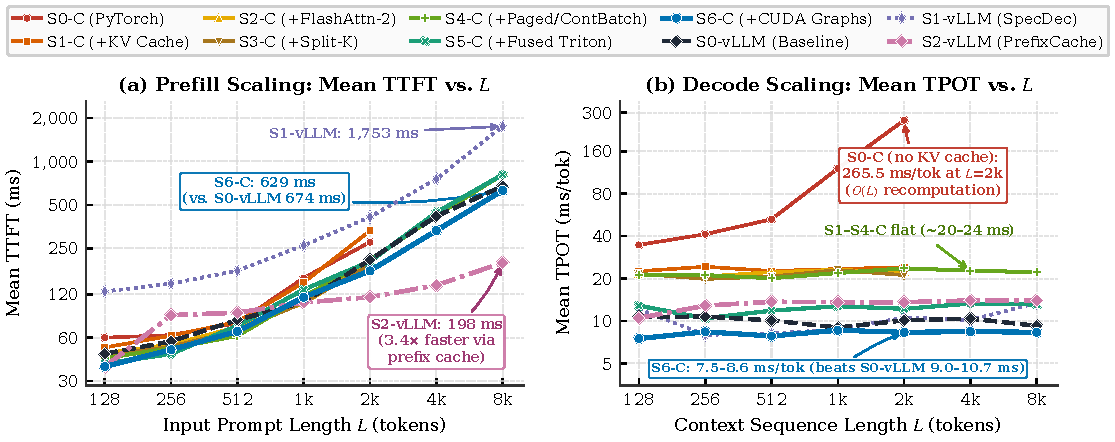
\includegraphics[width=\textwidth]{figures/fig2_context_scaling.pdf}
  \caption{Context-length scaling ($L \in [128, 8192]$, $C{=}1$, 64 output tokens). \textbf{(a)}~Mean TTFT shows FlashAttention-2 (\stage{S2-C}--\stage{S6-C}) matching or beating \stage{stage-0-vllm} ($629.3$ vs.\ $673.7$~ms at $L{=}8192$), while \stage{stage-2-vllm} cuts $L{=}8192$ TTFT $3.4\times$ to $198.3$~ms via prefix caching. \textbf{(b)}~Mean TPOT exposes \stage{S0-C}'s $O(S^2)$ blowup ($265.5$~ms at $L{=}2048$) vs.\ flat $7.50$--$8.60$~ms decoding in \stage{S6-C}.}
  \label{fig:context}
\end{figure*}

\subsection{Occupancy, Paged Memory \& Continuous Batching \texorpdfstring{(S3 $\rightarrow$ S4)}{(S3 to S4)}}
\textbf{Stage~2 $\rightarrow$ Stage~3 (Triton Split-K Decode).}
Following Flash-Decoding~\cite{dao2023flashdecoding}, \stage{stage-3-custom} introduces a two-stage Triton Split-K decode pipeline (\code{\_flash\_attention\_decode\_splitk\_fwd} + \code{\_flash\_attention\_splitk\_combine}, up to 32 splits) for $q_{\text{len}}{=}1$, partitioning $L_{\text{kv}}$ across parallel CTAs ($\text{grid}=(12, 15, 1)$) without $\text{BLOCK\_M}{=}16$ padding waste while retaining \code{\_flash\_attention\_fwd} for prefill. On \code{ncu} (Figure~\ref{fig:roofline}), Layer~0 decode attention drops $3.26\times$ ($129.44 \rightarrow 39.68~\mu$s combined; $32.06~\mu$s main pass = $4.04\times$), active warps jump $8.33\% \rightarrow 21.76\%$, DRAM bandwidth jumps $4.03\times$ ($16.41 \rightarrow 66.08$~GB/s), and total \code{nsys} attention GPU time collapses $6.54\times$ ($111.20 \rightarrow 17.00$~ms, $2.2\%$ of GPU time). Yet $C{=}1$ decode step barely moves ($25.19 \rightarrow 24.11$~ms) and serialized short-context runs ($C{=}2..16$) slightly regress ($-4.6\%$ to $-9.9\%$) because the extra combine kernel raises total launches to $74{,}220$ ($703.33$~ms CPU launch overhead, pushing GPU idle to $59.19\%$), while \code{asyncio.Lock} pins throughput flat at ${\sim}39$--$45$~tok/s and \code{torch.cat} KV appends cost $24.64~\mu$s per layer.

\textbf{Stage~3 $\rightarrow$ Stage~4 (Paged KV Cache \& Continuous Batching).}
\stage{stage-4-custom} eliminates request serialization and KV reallocation by implementing a physical KV block pool (\code{KV\_BLOCK\_SIZE=16}, 4,096 blocks), an in-place Triton \code{\_reshape\_and\_cache} scatter kernel, indirect \code{block\_table} attention gather, and an iteration-level continuous batching scheduler (\code{max\_batch\_size=64}, equal-length prefill grouping, batched $M{=}B$ decode, single batch \code{.tolist()} sampling D2H, and recomputation preemption)~\cite{kwon2023vllm,yu2022orca}.

The impact on concurrency scaling is transformative (Figure~\ref{fig:pareto}): aggregate throughput scales $32.7\times$ from $C{=}1$ ($38.51$~tok/s) to $1{,}260.39$~tok/s at $C{=}64$—already reaching $102.3\%$ of \stage{stage-0-vllm} ($1{,}232.26$~tok/s) with $4.95\times$ tighter P99 ITL ($52.30$ vs.\ $258.96$~ms). At $C{=}16$, throughput jumps $13.60\times$ over Stage~3 ($525.85$ vs.\ $38.67$~tok/s) and mean TTFT plunges $91\times$ ($47{,}151.62 \rightarrow 517.92$~ms). On \code{ncu}, \code{\_reshape\_and\_cache} cuts Layer~0 decode KV write $4.61\times$ ($24.64 \rightarrow 5.34~\mu$s), unlocking full $L{=}128..8192$ context sweeps ($22.20$~ms TPOT at $L{=}8192$). Nevertheless, single-stream decode remains severely host-bound: $72{,}933$ eager launches burn $669.98$~ms of CPU overhead ($53.53\%$ GPU idle), including $3{,}584$ \code{CatArrayBatchedCopy} launches from unfused \code{rotate\_half} RoPE alongside unfused RMSNorm, residual-add, and SwiGLU chains.

\subsection{Host-Dispatch Elimination: Fusion \& CUDA Graphs \texorpdfstring{(S5 $\rightarrow$ S6)}{(S5 to S6)}}
\textbf{Stage~4 $\rightarrow$ Stage~5 (Triton Operator Fusion).}
\stage{stage-5-custom} fuses the remaining elementwise chains into three custom Triton kernels plus merged MLP weights: (i)~\code{\_rms\_norm\_fwd} with fp32 variance and threaded residual-add fusion (\code{HAS\_RESIDUAL=True}), (ii)~in-place 4D-strided \code{\_rope\_embedding\_fwd} eliminating all \code{rotate\_half} slicing and \code{CatArrayBatchedCopy} calls, and (iii)~merged \code{gate\_up\_proj} linear weights (reducing per-layer linear calls from 7 to 6, matching vLLM's fused MLP width) paired with 2D-tiled \code{\_swiglu\_fwd}.

As Figure~\ref{fig:nsys} illustrates, total CUDA kernels drop $3.03\times$ ($72{,}933 \rightarrow 24{,}101$, with \code{CatArrayBatchedCopy} falling $3{,}584 \rightarrow 0$), CPU launch overhead drops $-45.57\%$ ($669.98 \rightarrow 364.68$~ms), non-linear/non-attention GPU time (\code{norm\_act\_other}) falls $-53.50\%$ ($137.74 \rightarrow 64.05$~ms), and GPU idle drops from $53.53\%$ to $28.97\%$. Consequently, \code{nsys} decode step time falls $-36.08\%$ ($19.68 \rightarrow 12.58$~ms), lifting $C{=}1$ throughput $+77.7\%$ ($38.51 \rightarrow 68.44$~tok/s, TPOT $14.19$~ms) and $C{=}64$ throughput to $1{,}486.13$~tok/s ($120.6\%$ of \stage{stage-0-vllm}). Still, with zero CUDA graphs, eager dispatch of the remaining $24{,}100$ launches (${\sim}376$/step) leaves $28.97\%$ GPU idle and a $1.91$~ms/step gap behind \stage{stage-0-vllm} ($10.67$~ms).

\begin{figure*}[t]
  \centering
  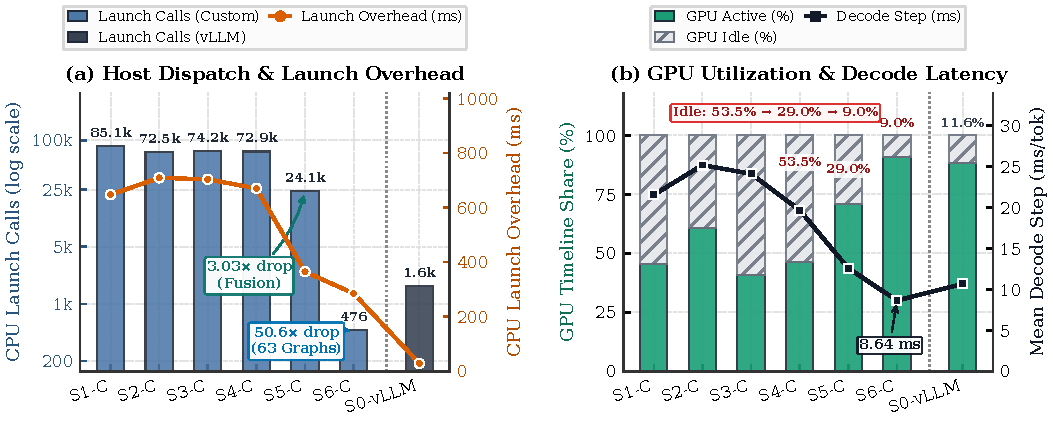
\includegraphics[width=\textwidth]{figures/fig3_nsys_bottleneck.pdf}
  \caption{Nsight Systems ($C{=}1$, 1024-in/64-out) host-dispatch and GPU utilization progression. \textbf{(a)}~Operator fusion (\stage{S5-C}) cuts CPU launch calls $3.03\times$ and bucketed CUDA graphs (\stage{S6-C}) cut them another $50.6\times$ to 476 calls (63 graph launches). \textbf{(b)}~GPU idle collapses from $53.5\%$ (\stage{S4-C}) to $29.0\%$ (\stage{S5-C}) to $9.0\%$ (\stage{S6-C}), yielding an $8.64$~ms decode step ($19.0\%$ faster than \stage{stage-0-vllm}'s $10.67$~ms).}
  \label{fig:nsys}
\end{figure*}

\textbf{Stage~5 $\rightarrow$ Stage~6 (Bucketed CUDA Graphs).}
\stage{stage-6-custom} introduces a \code{DecodeGraphRunner} that captures fixed-shape decode ($q_{\text{len}}{=}1$) into static \code{torch.cuda.CUDAGraph} buckets $B \in \{1, 2, 4, 8, 16, 32, 64\}$ while keeping variable-length prefill eager. To guarantee capture safety with zero host-device synchronization, the decode forward accepts a static integer \code{max\_context\_len} and masks padded lanes via \code{context\_lengths[pad] == 0} across KV scatter, RoPE, and Split-K attention.

Replaying 63 decode steps as CUDA graphs slashes \code{cpu\_launch\_calls} by $50.6\times$ ($24{,}100 \rightarrow 476$, $-98.02\%$), cuts CPU launch overhead $-21.78\%$ ($364.68 \rightarrow 285.25$~ms), collapses GPU idle $3.21\times$ ($28.97\% \rightarrow 9.03\%$, achieving $90.97\%$ active—higher than \stage{stage-0-vllm}'s $88.39\%$), and reduces \code{decode\_step\_avg\_ms} by $-31.32\%$ ($12.58 \rightarrow 8.64$~ms, $19.0\%$ faster than \stage{stage-0-vllm}'s $10.67$~ms). End-to-end, \stage{stage-6-custom} surpasses \stage{stage-0-vllm} at \emph{every} concurrency ($C{=}1$: $113.42$ vs.\ $87.77$~tok/s [$129.2\%$], TPOT $8.43$~ms; $C{=}16$: $1{,}065.51$ vs.\ $831.19$~tok/s [$128.2\%$]; $C{=}32$: $1{,}410.49$ vs.\ $966.96$~tok/s [$145.9\%$]; $C{=}64$: $1{,}770.61$ vs.\ $1{,}232.26$~tok/s [$143.7\%$], P99 ITL $27.57$ vs.\ $258.96$~ms) and \emph{every} context length $L \in [128, 8192]$ ($7.50$--$8.60$~ms TPOT, $102.3\%$--$140.7\%$ of vLLM throughput). Across Stages~0$\rightarrow$6, $C{=}1$ throughput improved $7.60\times$, $C{=}16$ throughput improved $72.93\times$, and $L{=}2048$ TPOT improved $31.95\times$.

\begin{figure*}[t]
  \centering
  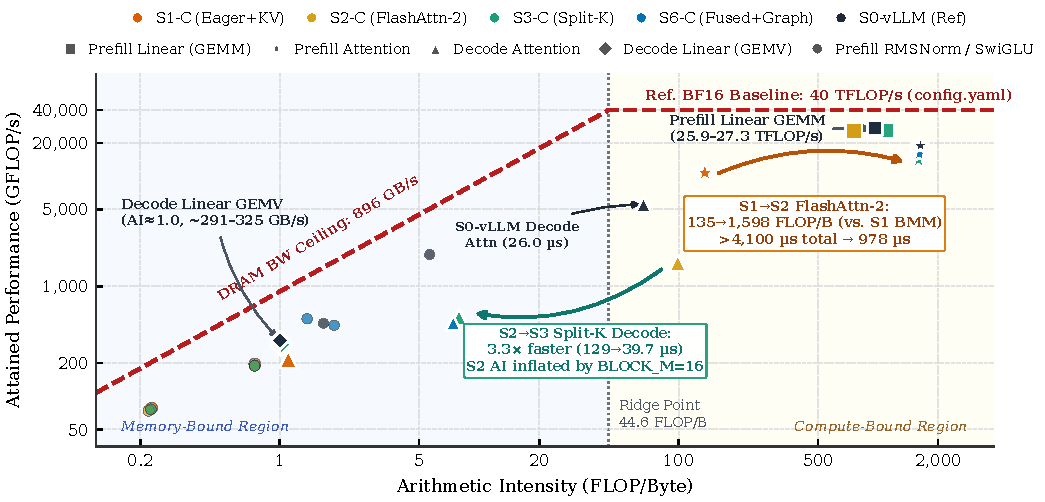
\includegraphics[width=0.95\textwidth]{figures/fig4_roofline.pdf}
  \caption{RTX~5080 Laptop (\code{sm\_120}) Layer~0 hardware roofline from Nsight Compute (\code{ncu}) against physical ceilings ($896$~GB/s DRAM, $40$~TFLOP/s BF16 Tensor, ridge $44.6$~FLOP/B). Highlights the $11.8\times$ prefill attention AI leap (\stage{S1-C}$\rightarrow$\stage{S2-C}), $4.0\times$ Split-K decode attention speedup (\stage{S2-C}$\rightarrow$\stage{S3-C}), and \stage{S6-C} matching \stage{S0-vLLM}'s linear GEMM/GEMV roofline.}
  \label{fig:roofline}
\end{figure*}

% ============================================================================
\section{Serving-Level Trade-offs on vLLM (Track A)}
% ============================================================================

To complement the kernel- and runtime-level progression of Track~B, Track~A isolates two high-level serving optimizations directly on top of frozen \stage{stage-0-vllm}. Table~\ref{tab:vllm} summarizes their trade-offs.

\begin{table}[t]
\centering
\caption{Track~A feature isolation on vLLM~0.31.0 ($\Delta$ vs.\ \stage{stage-0-vllm}). Speculative decoding helps only at $C \le 2$ and regresses at scale; prefix caching dominates high concurrency and long contexts.}
\label{tab:vllm}
\scriptsize
\setlength{\tabcolsep}{1.8pt}
\begin{tabular}{@{}l rrr@{}}
\toprule
\textbf{Metric} & \textbf{S0-vLLM} & \textbf{S1-vLLM} & \textbf{S2-vLLM} \\
& (Baseline) & (SpecDec) & (PrefixCache) \\
\midrule
$C{=}1$ Tput (tok/s)       & 87.77 & \textbf{105.97} (+20.7\%) & 80.35 (-8.5\%) \\
$C{=}1$ P50 ITL (ms)       & \textbf{10.91} & 42.86 ($3.93\times$) & 13.00 (+19.2\%) \\
$C{=}64$ Tput (tok/s)      & 1,232.26 & 872.47 (-29.2\%) & \textbf{2,874.36} (+133\%) \\
$C{=}64$ TTFT (ms)         & 896.18 & 1,770.88 (+97.6\%) & \textbf{228.52} (-74.5\%) \\
$C{=}64$ P99 ITL (ms)      & 258.96 & 392.65 (+51.6\%) & \textbf{44.42} (-82.8\%) \\
$L{=}8192$ TTFT (ms)       & 673.66 & 1,752.66 (+160\%) & \textbf{198.30} (-70.6\%) \\
\code{nsys} Launch (ms)    & \textbf{28.90} & 277.00 ($9.58\times$) & 29.96 (+3.7\%) \\
\code{nsys} GPU Idle (\%)  & \textbf{11.61} & 35.27 ($3.04\times$) & 13.09 (+1.5pp) \\
\code{ncu} Dec Linear AI   & 1.001 & \textbf{15.473} ($15.5\times$) & 1.007 \\
\bottomrule
\end{tabular}
\end{table}

\subsection{Speculative Decoding Limits (\texorpdfstring{\stage{stage-1-vllm}}{stage-1-vllm})}
In \stage{stage-0-vllm}, Layer~0 \code{ncu} confirms that single-token decode linear projections are strictly memory-bandwidth bound ($\text{AI}{=}1.001$~FLOP/B, $321.10$~GB/s, $0.321$~TFLOP/s). \stage{stage-1-vllm} pairs the 1.54B target with a 0.49B draft model ($K{=}5$)~\cite{leviathan2023speculative,chen2023speculative} to verify $M{=}K{+}1{=}6$ tokens in parallel. At the kernel level, the hypothesis succeeds decisively: \code{Decode Linear} arithmetic intensity jumps $15.5\times$ ($1.001 \rightarrow 15.473$~FLOP/B) and attained compute rises $15.7\times$ ($0.321 \rightarrow 5.037$~TFLOP/s) with ${\sim}98.2\%$ token acceptance ($L_{\text{acc}} \approx 5.91$).

End-to-end, however, speedup caps at $+20.7\%$ at $C{=}1$ ($105.97$ tok/s, TPOT $-23.1\%$ to $8.38$~ms) and $+7.5\%$ at $C{=}2$, then \emph{regresses} $-20.2\%$ to $-29.2\%$ for $C \ge 4$ ($872.47$~tok/s at $C{=}64$). Profiling reveals three compounding causes: (1)~an unfavorable draft-to-target size ratio ($0.49\text{B}/1.54\text{B} \approx 1/3$), meaning $K{=}5$ sequential memory-bound draft steps already cost ${\sim}1.67\times$ a target decode step; (2)~a $9.58\times$ surge in host orchestration overhead ($28.90 \rightarrow 277.00$~ms, $1{,}636 \rightarrow 19{,}843$ CPU calls, CUDA graph launches dropping $63 \rightarrow 13$), widening GPU idle from $11.61\%$ to $35.27\%$; and (3)~bursty multi-token SSE flushing that inflates $C{=}1$ P50 ITL $3.93\times$ ($10.91 \rightarrow 42.86$~ms).

\subsection{Automatic Prefix Caching Gains (\texorpdfstring{\stage{stage-2-vllm}}{stage-2-vllm})}
At $C{=}64$ in \stage{stage-0-vllm}, redundant 512-token prefills cause mean TTFT to explode $12.2\times$ ($73.31 \rightarrow 896.18$~ms, P99 $3{,}889.86$~ms) and interrupt active decode batches (P99 ITL $258.96$~ms). Enabling \code{--enable-prefix-caching} (\stage{stage-2-vllm}, RadixAttention~\cite{zheng2024sglang}) reuses shared-prefix KV blocks in $O(1)$ time with virtually zero host dispatch penalty ($29.96$~ms launch overhead, $1{,}636$ calls, 63 CUDA graphs). At $C{=}64$, aggregate throughput surges $+133.3\%$ ($2.33\times$) to $2{,}874.36$~tok/s, mean TTFT drops $-74.5\%$ ($228.52$~ms), P99 TTFT drops $-68.8\%$ ($1{,}211.93$~ms), TPOT halves ($45.15 \rightarrow 20.57$~ms), and P99 ITL collapses $-82.8\%$ ($44.42$~ms). At $L{=}8192$ ($C{=}1$), TTFT drops $-70.6\%$ ($673.66 \rightarrow 198.30$~ms), lifting throughput $+16.5\%$ to $59.36$~tok/s. The sole trade-off is a modest $-8.5\%$ to $-26.5\%$ radix bookkeeping tax at low concurrency ($C \le 8$), cleanly shifting the system bottleneck from prefill compute serialization to the GDDR7 decode bandwidth ceiling.

% ============================================================================
\section{Discussion \& Limitations}
% ============================================================================

\textbf{Why \stage{stage-6-custom} Surpasses Baseline vLLM.}
Our Layer~0 \code{ncu} data (Figure~\ref{fig:roofline}) show that \stage{stage-6-custom} and \stage{stage-0-vllm} operate at virtually identical kernel efficiency: prefill linear GEMM attains $27.21$ vs.\ $27.35$~TFLOP/s, and decode linear GEMV attains $321.39$ vs.\ $321.10$~GB/s ($0.323$ vs.\ $0.321$~TFLOP/s). Because both engines execute the same underlying cuBLAS GEMMs/GEMVs and comparable fused Triton/FlashAttention kernels, \stage{stage-6-custom}'s end-to-end advantage ($129.2\%$ at $C{=}1$, $143.7\%$ at $C{=}64$) stems primarily from \emph{lower runtime and scheduling overhead}: (i)~as a single-model engine without vLLM's generalized multi-worker IPC, tokenizer/detokenizer abstraction layers, or block-table manager overhead, \stage{stage-6-custom} sustains a $19.0\%$ faster decode step ($8.64$ vs.\ $10.67$~ms) and lower GPU idle ($9.03\%$ vs.\ $11.61\%$); and (ii)~grouping equal-length prefills separately from pure bucketed decode steps eliminates the mixed chunked-prefill/decode scheduling jitter that drives \stage{stage-0-vllm}'s $258.96$~ms P99 ITL at $C{=}64$ (vs.\ $27.57$~ms in \stage{stage-6-custom}).

\textbf{Limitations \& Threats to Validity.}
This study intentionally trades production generality for experimental isolation. First, \stage{stage-6-custom} is a single-GPU, single-architecture (\code{Qwen2}) BF16 engine; unlike vLLM, it lacks tensor/pipeline parallelism, quantization (FP8/AWQ/GPTQ), LoRA adapters, chunked prefill, and prefix caching (hence \stage{stage-2-vllm} still leads at $C{=}64$ with $2{,}874.36$~tok/s). Second, our closed-loop sweeps use a fixed homogeneous prompt length per run, which favors both equal-length prefill grouping in \stage{stage-4..6-custom} and prefix caching in \stage{stage-2-vllm}; heterogeneous prompt lengths in production would require chunked prefill to bound ITL spikes. Third, measurements were collected on a consumer laptop GPU under WSL2, where dynamic thermal/clock scaling causes sustained DRAM bandwidth (${\sim}321$~GB/s in \code{ncu}) to sit below the nominal $896$~GB/s physical ceiling, and NCU tensor FLOPs are estimated via instruction counts ($\text{inst} \times 4096$).

% ============================================================================
\section{Conclusion \& Future Work}
% ============================================================================
Through a reproducible 10-stage empirical study on an RTX~5080 Blackwell laptop GPU, we demonstrated that LLM inference optimization is fundamentally a sequence of \emph{bottleneck handoffs}. Eliminating $O(S^2)$ decode recomputation (Stage~1) flips GPU idle from $8.9\%$ to $54.3\%$; tiling prefill attention with FlashAttention-2 (Stage~2) boosts prefill AI $11.8\times$ but starves decode SMs until Split-K parallelization (Stage~3); paged continuous batching (Stage~4) unlocks $32.7\times$ concurrency scaling while exposing $72{,}933$ eager launches; and only combining Triton operator fusion (Stage~5) with bucketed CUDA graphs (Stage~6) collapses GPU idle to $9.03\%$ and surpasses baseline vLLM~0.31.0 across all tested concurrencies and context lengths. In future work, we plan to add radix prefix caching to \code{custom-serving/}, evaluate high-ratio speculative decoding (e.g., 14B-AWQ target with a 0.5B draft), and explore native Blackwell \code{sm\_120} FP8/FP4 quantized decode kernels.

\bibliographystyle{unsrtnat}
\bibliography{references}

\end{document}
